% !TEX TS-program = lualatex
% !TEX encoding = UTF-8 Unicode
% --- Preamble: Styling ---
\documentclass[a4paper,12pt]{article}
\usepackage[left=3cm,top=3cm,bottom=2cm,right=2cm]{geometry}

% Encoding & Language
\usepackage[utf8]{inputenc}
\usepackage[T1]{fontenc}
\usepackage[portuguese]{babel}
\addto\extrasportuguese{\renewcommand{\contentsname}{Índice}}

% Margins, Columns, Indentation & Spacing
\usepackage{multicol}
\usepackage{indentfirst}
\usepackage{ragged2e}  % For extendability
\usepackage{setspace}
\onehalfspacing
\setlength{\columnsep}{1cm}

% Headers, Titles, Footnotes & Captioning
\usepackage{sectsty}
\usepackage{titling}
\renewcommand\maketitlehooka{\null\mbox{}\vfill}
\renewcommand\maketitlehookd{\vfill\null}
\usepackage{footmisc}
\usepackage{caption}
\captionsetup[figure]{font=footnotesize}

% Graphics Support
\usepackage{graphicx}
\graphicspath{{./assets/}}
\usepackage{svg}
\usepackage{tikz}
\usepackage{float}
\usepackage{fancyhdr}
\usepackage{xcolor}
\usetikzlibrary{shapes,shadows,arrows,positioning,calc}
\tikzstyle{RectObject}=[rectangle,fill=white,draw,line width=0.5mm]
\tikzstyle{line}=[draw]
\tikzstyle{arrow}=[draw, -latex]

% --- Preamble: Commands ---
\pagestyle{fancy}
\fancyhf{}
\fancyfoot[R]{\thepage}
\renewcommand{\headrulewidth}{0pt}

% --- Document: Begin ---
\begin{document}
% --- Document: Title Page ---
\begin{titlingpage}
    \begin{center}
        {\large
            % Institution
            {\Huge
                FATEC -- Prof. Waldomiro May
            }\\
            ANÁLISE E DESENVOLVIMENTO DE SISTEMAS

            % Project Presentation
            \vspace{1cm}
            SEMANA DE TECNOLOGIA

            % Project Logo
            \vspace{6cm}
            \raisebox{-0.75em}{
\includegraphics[scale=0.1]{neotasker-logo.png}}
            % Project Name
            {\Huge
                \textbf{NeoTasker}
            }

            % Project Description
            Agenda Pessoal

            % Authors
            \vspace{2cm}
            CHRYSTIAN M. FRANKLIN \\
            WELLINGTON E. RODRIGUES

            % Date
            \vspace{8cm}
            2023.2
        }
    \end{center}
\end{titlingpage}

% --- Document: Table of Contents ---
\tableofcontents
\pagebreak

% --- Document: Table of Figures ---
\listoffigures
\pagebreak

% --- Document: Content ---
% --- Segment: Introduction ---
\section{Introdução}
\subsection{Tema}
O software \textbf{NeoTasker} é um \textit{Sistema de Gerenciamento de Agenda Pessoal}. Este caracteriza-se pelo controle de atividades e eventos decorrentes do dia-a-dia de um indivíduo.

\subsection{Justificativa de Escolha do Tema}
A organização pessoal é uma tarefa árdua e frequentemente mais complexa do que imaginada, especialmente quando é considerado as rotinas frenéticas de estudantes e trabalhadores, devido ao seu vasto e variado uso de tempo, com suas rotinas crescentemente mais corridas.

A partir dessa consideração, o tema de \textbf{agenda pessoal} foi selecionado devido à familiaridade do ambiente dos autores, em conjunto com as possibilidades de diferentes soluções relacionadas ao aspecto de controle de tempo e organização de rotinas.

\subsection{Descrição do Problema}
O sistema deve ser capaz de efetuar o agendamento, modificação, consultas e remoção dos diferentes tipos de atividades presentes de maneira individual. Além de apresentar relatórios e informações estatísticas sobre as atividades e o uso do sistema, visando melhorar a experiência do usuário em relação a sua organização de tempo.

\subsection{Objetivos do Projeto}
Este projeto é caracterizado por ser uma atividade conjunta com o objetivo de desenvolver os conteúdos das seguintes disciplinas do segundo período do curso de análise e desenvolvimento de sistemas:
\begin{itemize}
    \item \textbf{IES100:} Engenharia de Software I;
    \item \textbf{IHC001:} Interação Humano Computador;
    \item \textbf{ILP010:} Linguagem de Programação;
    \item \textbf{ISI002:} Sistemas de Informação.
\end{itemize}

Além do aspecto disciplinar, este projeto tem como objetivos secundários o desenvolvimento de habilidades essenciais no atual ambiente de trabalho:
\begin{itemize}
    \item A produção de um projeto relacionado ao \textbf{Gerenciamento de Tempo e Rotina};
    \item A execução da \textbf{Metodologia Ágil} e \textbf{SCRUM};
    \item A \textbf{Análise de Projetos} e o \textbf{Levantamento de Requisitos};
    \item A \textbf{Consideração de Aspectos de Acessibilidade};
    \item A \textbf{Produção de Documentação e Manuais};
    \item O \textbf{Desenvolvimento de Sistemas de Softwares Completos};
    \item A \textbf{Implementação de Caso de Testes}.
\end{itemize}

\subsection{Organização do Projeto}
\subsubsection{Estrutura do Projeto}
O projeto está estruturado a partir da organização de projetos em cascatas, com base na seguinte visão:

\vspace{1em}
\begin{figure}[H]
    \centering
    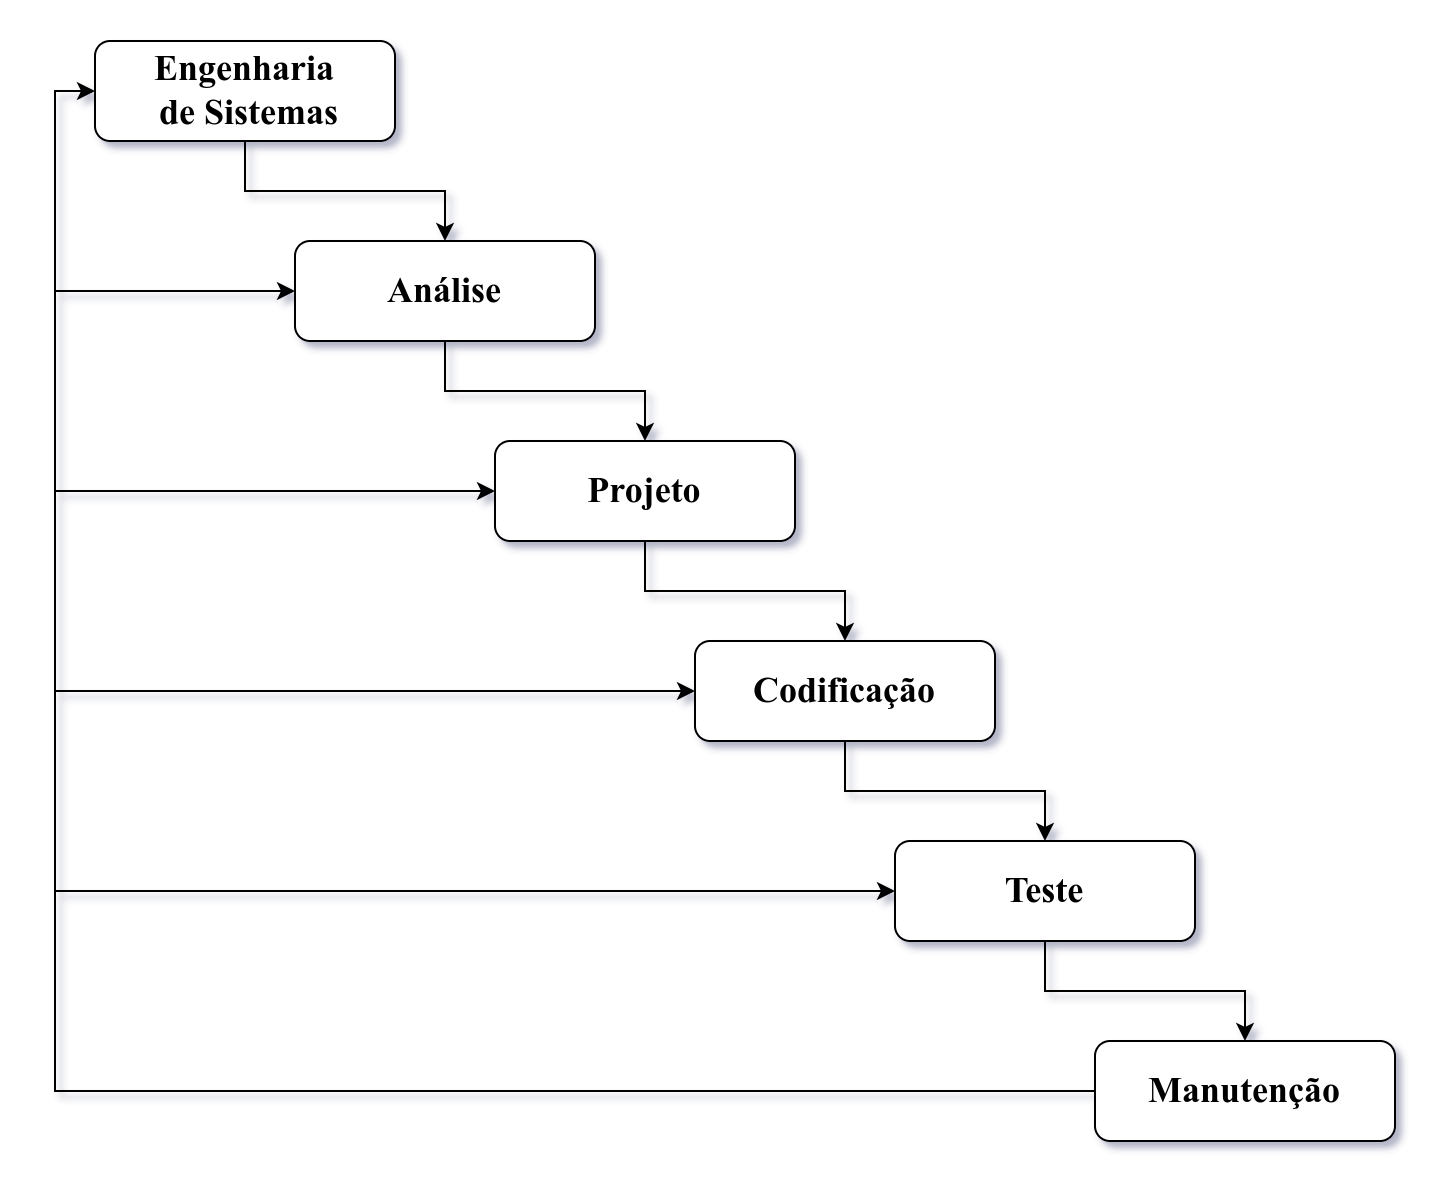
\includegraphics[scale=0.25]{waterfall.drawio.png}
    \caption{Desenvolvimento em Cascata}
\end{figure}

Esta estrutura é o que permite que o desenvolvimento ocorra de maneira crescente e parcial, onde cada adição, extensão, modificação ou remoção de componentes resulte na adaptação da documentação e código, voltando ao ponto de desenvolvimento no qual a mudança ocorreu, garantindo assim uma maior estabilidade e qualidade de produto.

\subsubsection{Método de Trabalho}
O Método Ágil com SCRUM\footnote{
    Criado por \textbf{Jeff Sutherland} em 1990.
} foi empregado para orientar os desenvolvimentos dos diferentes processos presentes na estrutura do projeto. Utilizado também no mercado de trabalho, o método incorpora as atividades de levantamento de requisitos, análise, projetos \textit{(prototipação)}, implementação/evolução, e entrega.

As atividades individuais são organizadas em \textbf{Sprints}, que delimitam um certo período de tempo -- \textit{geralmente de uma a duas semanas} -- desde o início até o fim do processo.

\subsubsection{Divisão de Responsabilidades}
O projeto consta com dois membros, portanto, as atividades estão substituídas da seguinte maneira:

\paragraph{Chrystian M. Franklin}
\begin{itemize}
    \item Planejamento e Estruturação do Projeto;
    \item Construção de Documentação e Manuais;
    \item Controle do Versionamento;
    \item Correção de Bugs e Otimizações;
    \item Implementação de Casos de Testes Automatizados;
    \item Desenvolvimento dos Aspectos Back-End.
\end{itemize}

\paragraph{Wellington E. Rodrigues}
\begin{itemize}
    \item Design e Padrões de Cores;
    \item Organização e Distribuição de Atividades e Responsabilidades;
    \item Levantamento de Requisitos e Features Adicionais;
    \item Consideração de Itens de Acessibilidade;
    \item Construção de Diagramas e Protótipos Gráficos;
    \item Desenvolvimento dos Aspectos Front-End.
\end{itemize}

% --- Segment: Requirements ---
\section{Requisitos}
% --- Document: End ---
\end{document}
